\documentclass{scrartcl}
\title{\rmfamily Software Engineering -- Blatt 8}
\author{Rasmus Diederichsen \and Felix Breuninger\and 
   \texttt{\{rdiederichse, fbreunin\}@uos.de}
}
\date{\today}
\usepackage[ngerman]{babel}
\usepackage[space]{grffile} % for spaces in includegraphics fnames
\usepackage{marvosym, microtype, textcomp, xifthen, multirow, booktabs, dingbat,
   titlesec, enumitem, fullpage, tikz, IEEEtrantools, array, amsmath, listings,
amssymb, graphicx, subcaption, lmodern,pgfplots}
\usepackage[pdftitle={Software Engineering -- Blatt 8}, 
   pdfauthor={Rasmus Diederichsen, Felix Breuninger}, 
   hyperfootnotes=true,
   colorlinks,
   bookmarksnumbered = true,
   linkcolor = lightgray,
   plainpages = false,
citecolor = lightgray]{hyperref}
\usepackage[utf8]{inputenc}
\usepackage[T1]{fontenc}
\usepackage[all]{hypcap}
\titleformat{\section}[hang]{\bf}{Aufgabe 8.\arabic{section}:}{1em}{}[]
\titleformat{\subsection}[hang]{\bf}{\hspace{1em}\alph{subsubsection})}{1em}{}[]

\lstset{
   frame=single,
   basicstyle=\ttfamily\small,
   frameround=tttt,
   backgroundcolor=\color{lightgray!10},
   keywordstyle=\color{teal}\textbf,
   stringstyle=\itshape,
   showstringspaces=false,
   language=[gnu] make,
   morecomment=[n]{$(}{)},
   commentstyle=\color{blue},
   title=\lstname
}
\usetikzlibrary{shapes,positioning,calc,decorations.text,graphs,arrows.meta}
\begin{document}

\fontfamily{ptm}\selectfont
\maketitle

\section{Klassendiagramm}

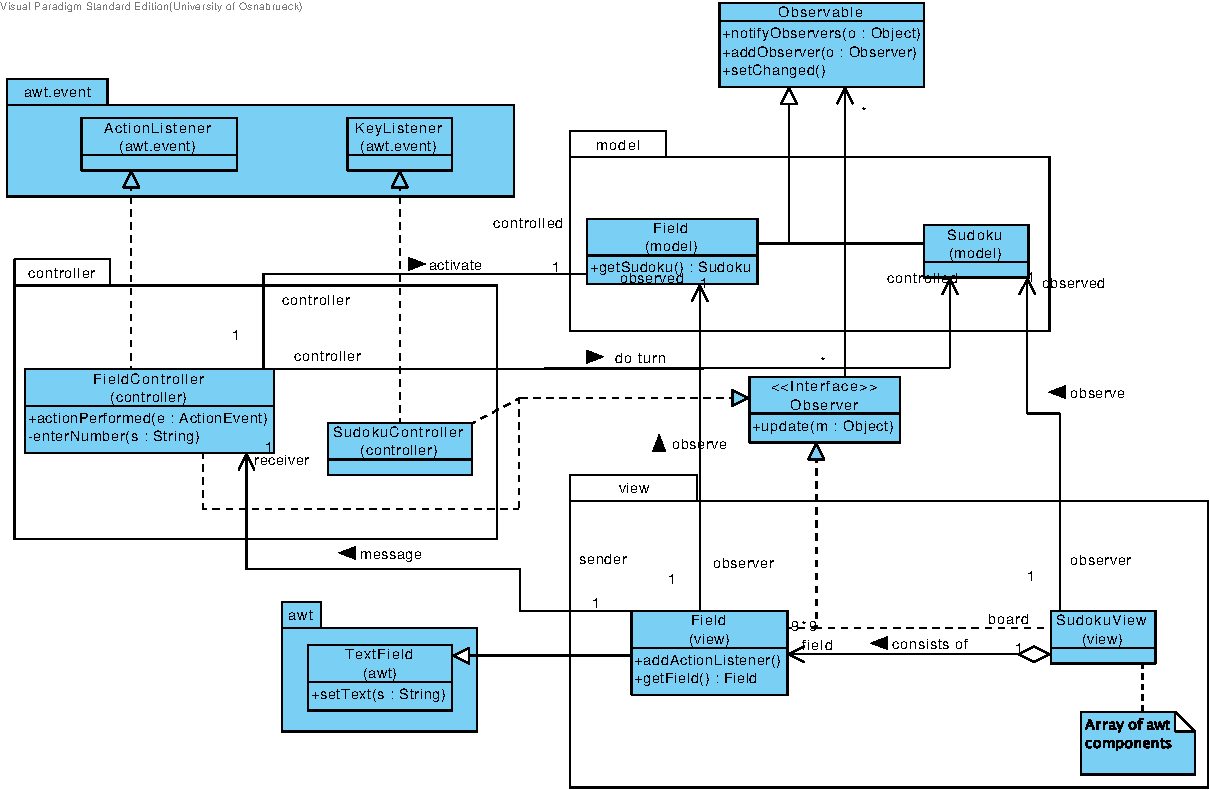
\includegraphics[width=\linewidth]{Sudoku-MVC.pdf}

\section{Sequenzdiagramm}

Frag mich, woher der Pfeil oben links kommt. Dafuq.

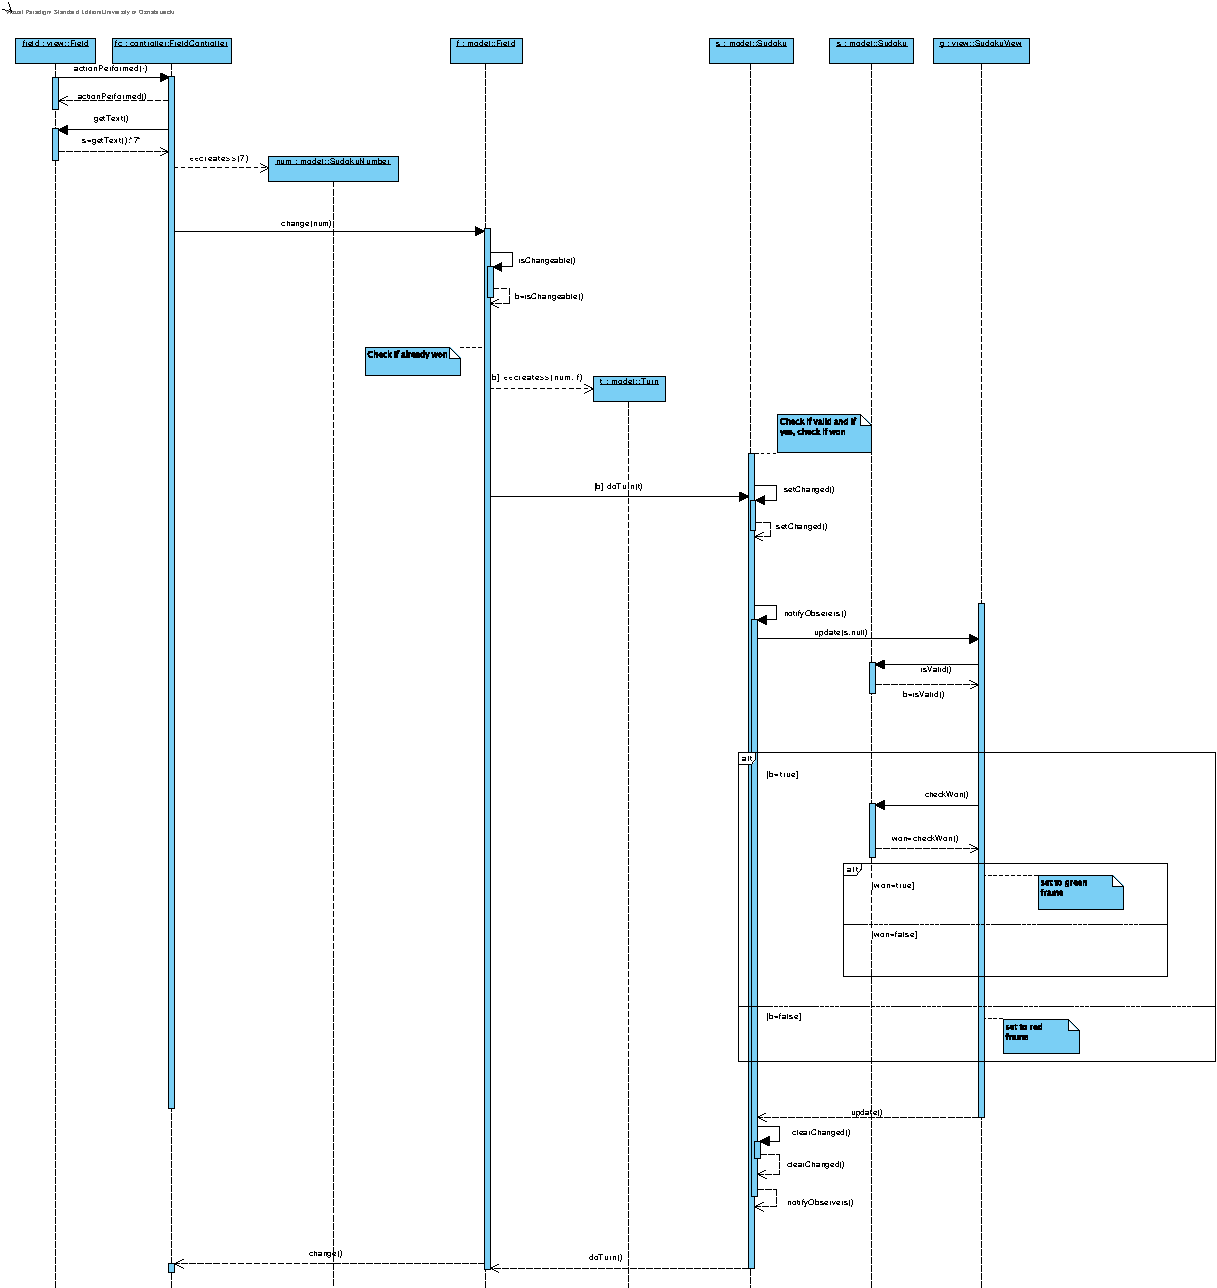
\includegraphics[width=\linewidth]{Sudoku-SD.pdf}

\section{Kommunikationsdiagramm}

\emph{Anmerkung:} Wie aus den Kommentaren ersichtlich, produziert Visual
Paradigm hier teilweise Nachrichten, die nicht der im Sequenzdiagramm
hinterlegten Semantik entsprechen.

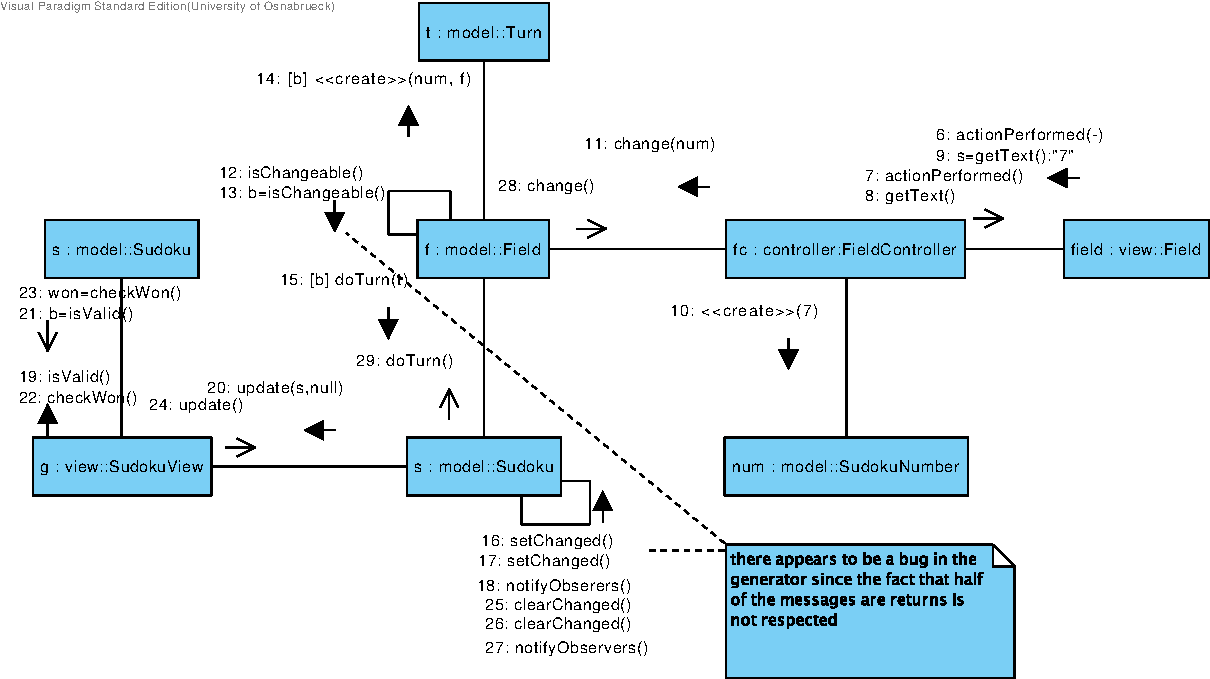
\includegraphics[width=\linewidth]{Sudoku-SD - Communications.pdf}

\section{Objektdiagramm}

\section{Zustandsdiagramm}

\end{document}
